\documentclass[11pt]{article}
\usepackage{multicol}
\usepackage{url}
\usepackage{graphicx}
\usepackage{natbib}
\usepackage{amsmath}
\usepackage{paralist}
\usepackage[small]{titlesec}
\usepackage[title]{appendix}
\begin{document}
\title      {\vspace{-2cm}\textbf{Individual Selection with Mutation for Cooperative Group Formation}}
\author	    {Thomas Smith\\taes1g09@ecs.soton.ac.uk}
\date       {\today}
\maketitle
\section{Introduction}
% 1.5 pages
% o   Introduction: You need not spend more than 1.5 pages describing the original paper.
% ?         briefly describe the paper/experiment
% ?         What you evolved including
% ?         How you represented individuals
% ?         What fitness function did you define
% ?         What kind of GA you used
% ?         Steady state/ generational?  Tournament selection/ fitness proportionate (roulette wheel)?
% ?         What kind of crossover (if any) you used.
% ?         All parameters (enough detail so a reader could re-implement the GA)

%basic introduction
\citet*{orig} show that environmental conditions need not be externally imposed in order to promote the evolution of cooperative traits. They present a model which permits suitable conditions to arise via individual selection, and show that even in environments that initially select for selfish behaviour, a niche construction process can allow for cooperative behaviours to be ultimately successful. This paper reimplements the algorithm described, and extends the model to show not only that the process is accelerated by the introduction of mutation to the model, but also that a side-effect of the niche construction process then favours selecting against individuals that are able to mutate, resulting in a more stable niche.




\section{Reimplementation}
%description of original paper
In \citet{orig}, an algorithm is presented which demonstrates that under the right circumstances, individuals can select for environments that promote cooperation. Using the trait-group aggregation and dispersal model presented in \citet{wilson}, individuals are permitted to select for control both over individual strategy and initial group size. Large groups receive a resource bonus~\citep{allee}, but are also more susceptible to exploitation by selfish individuals. Groups are formed according to individual size preferences, and with a random but globally proportionate composition of strategies. Individuals in groups are then reproduced over a number of generations, with shares of the group's resources ($r_i$) allocated according to the proportion of individuals with a particular genotype within that group. When using the parameters in Appendix~\ref{app:parameters}, this should result in individuals selecting away from the resource bonus of the larger groups in favour of an environment where the cooperative trait has greatest individual fitness. In small groups, stochastic between-group variation ultimately globally favours the growth of groups with a higher proportion of cooperative individuals.

After initialising the migrant pool with $N$ individuals, \citet{orig} present the following algorithm as an implementation of the trait-aggregation model. The steps represent a single cycle, and should be repeated for $T$ generations.\\
\begin{compactenum}
\item\textbf{Aggregation:} Assign individuals in the migrant pool randomly to groups according to their size preference - each group will have a random composition of strategies, but the average should be proportionate to the global ratios. Surplus individuals may be discarded.
\item\textbf{Reproduction:} Perform reproduction within groups - eq. \ref{eq:desire} gives the resource share that each genotype population receives, and eq. \ref{eq:shares} gives the resulting change in population size. Repeat for $t$ generations.
\item\textbf{Dispersal:} Return the progeny of each group
to the migrant pool.
\item\textbf{Scaling:} Rescale the migrant pool
back to size $N$, retaining the proportion of individuals with each genotype.
\end{compactenum}

\begin{align} \label{eq:desire}
  r_i &= \frac{n_iG_iC_i}{\sum\limits_{j}(n_jG_jC_j)}R
\end{align}
\begin{align} \label{eq:shares}
  n_i(t+1) &= n_i(t) + \frac{r_i}{C_i} - Kn_i(t)
\end{align}

\subsection{Representation}
In the reimplementation, individuals are represented as aggregate populations by genotype. Each individual can specify two genes: one for size, and one for strategy, and each gene can take one of two values, large/small and cooperative/selfish, respectively. This results in four possible genotypes, and so a migrant pool is maintained of the total count of each of the four types. Each group formed also maintains only the total count of each genotype within it, and aggregation, reproduction, dispersal and scaling operations are all carried out by population rather than individually.


The algorithm has no explicit fitness function - rather, an individual's fitness may be approximated by the total resource share of its genotype within the population as a whole. There is no crossover, but the algorithm could be said to be generational, as after each aggregation/dispersal round the whole population is rescaled back to a nominal `carrying capacity' ($N$). The rescaling can force populations below their minimum group sizes and hence to extinction when they are significantly outcompeted.\\
%TODO: write more here
\newpage
\subsection{Results}
% ~1 page
% o   Reimplementated Results (~1 page)
% ?         The reimplemented figures (side by side with the originals)
% ?         Discussion of what the results show/don't show, what worked/didn't work, what you learned
When the reimplemented algorithm is run using the parameters in Appendix~\ref{app:parameters}, the output closely follows the original findings (Figures~\ref{fig:original} and~\ref{fig:equalplot}).
\vspace{-.5cm}
\begin{figure}[!ht]
  \centering
  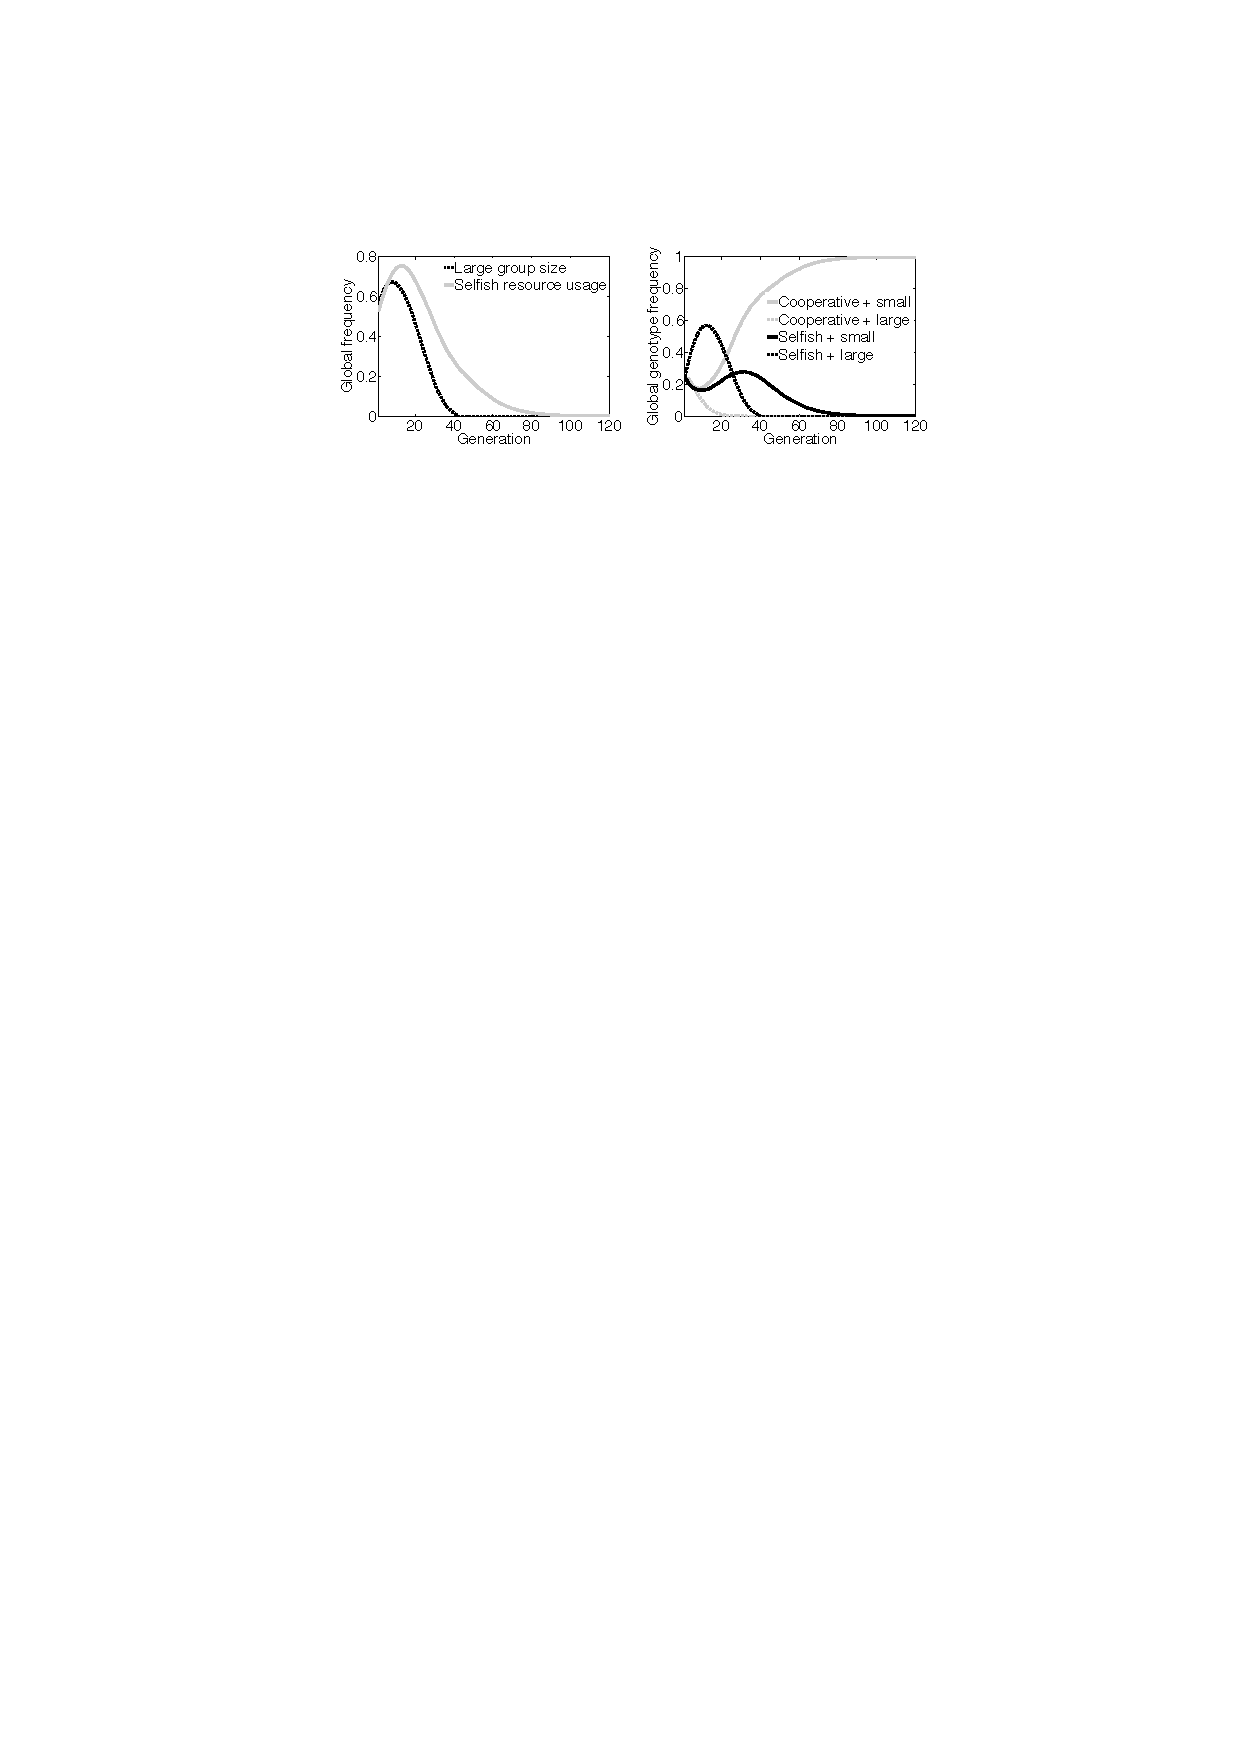
\includegraphics[scale=1.25]{original.pdf}
  \caption{Left: average environment and strategy through time. \newline Right: change in genotype frequencies over time. \citep{orig} }
  \label{fig:original}
\end{figure}

\begin{figure}[!ht]
  \centering
  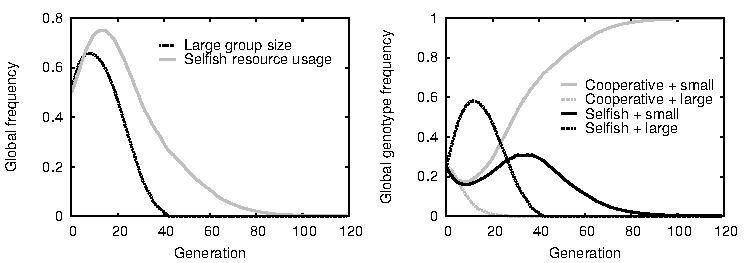
\includegraphics{equalplot.pdf}
  \caption{Results provided by reimplemented algorithm, as above. The plots match to a high degree of accuracy, showing accurate reimplementation. 
  }
  \label{fig:equalplot}
\end{figure}

%\small{(Note: both left plots display total population sizes of the large and selfish alleles, rather than the group size and resource usage as labelled.)}
As in \citet{orig}, large individuals initially benefit from the resource bonus, with large + selfish individuals flourishing as expected for the first few generations. Without a healthy population of large + cooperative individuals to exploit, the selfish individuals begin to decrease in frequency. Among the small groups, between-group variance exerts a selective pressure against groups containing selfish individuals \citep{Watson2011}, eventually driving the selfish allele extinct and allowing the cooperative + small genotype to fix in the population at equilibrium.

% All of the other genotypes eventually die out permanently due to being outcompeted for resources (mention across and between groups variance) and then being scaled away in step 7[TODO: check]
\clearpage
\section{Extension}
% ~1 page
% o   Describe your extension  (another page)
% ?        What is your research question/hypothesis?
% ?         e.g., 'compare x with y' or 'add x and see what difference it makes compared to not(x)'.
% ?         Describe methods
% ?         Any advancements you made
% ?         Support the value of asking that question (using literature)
% ?         What do you expect to happen (what might happen)?
% ?         Why do you think that?

%choice of extension
% a number of extensions of the original paper exist
% \citet{thesis} recommends altering the numebr of generations before breeding, or restiriction miigrations
% thise papers have done these things


The original result can be shown to be quite robust: even in the case of severe imbalance in the initial genotype distribution, it is generally seen that the cooperative + small genotype successfully forms a niche and eventually fixes (Appendix~\ref{app:graphs}, figure~\ref{fig:unevenplot}). However, this is only possible when there exists a critical minimum population of cooperative + small individuals that between-groups variation can select in favour of. In the model as presented, if a particular genotype dies out or does not exist in the initial distribution, then it is never possible for it to (re)enter the gene pool. In certain situations, this can be seen as disadvantageous  - for example, if in the original model the cooperative + small individuals were able to form large groups again once the selfish allele had been eradicated, then they could reap the resource bonus without exploitation by selfish individuals.

As an extension to the original model, this paper then presents analysis of cases where individuals may occasionally spontaneously change their size preference or strategy. An additional gene is introduced to each individual which both controls and is subject to these spontaneous changes, in a manner similar to a low rate of mutation across the whole population \citep{adaption}. The expectation is that the addition of mutable individuals will make the niche construction process possible in a wider range of more initially hostile populations.
%TODO: specify the actual question
\subsection{Representation}
Once again, individuals are represented by genotype as populations of identical clones. As there are three distinct genes, there are now eight separate combinations of alleles representing populations in the migrant pool and in each group. The reproduction code has been modified to respect the possibility of newly mutated individuals present in a group size different to that specified by their genotype. Mutation potentially occurs after each within-group reproduction cycle.

\citet{optimal} notes that `optimal per-locus mutation rates depend mainly on $1/L$ (the reciprocal of the genotype length)'. In this model, the length of each individual's genotype is 3, and a mutation rate of $1/3$ is high enough to cause no significant solution to arise. %I don't like the end of the sentence
However, the original reasoning behind the heuristic leads to a more effective value for mutation within the model. The use of a mutation rate of $1/L$ is intended to result in an average of one change to one gene in an individual per reproduction - in the model presented, the desired mutation rate is on the order of one change of one group per cycle of reproduction, and so a value of $1/num\_groups$ is more appropriate. Though the actual number of groups fluctuates based on prevailing group size preference, 550 groups may be taken as a reasonable approximation\footnote{~using the parameters in table~\ref{table:param} with equal distribution of genotypes: $\frac{2000}{40} + \frac{2000}{4} = 550$}. A mutation rate $M$ of $\frac{1}{550} \approx 0.002$ is therefore used throughout the rest of the paper.
\subsection{Results}
% ~1.5 pages
% o   Results of extension (another 1.5 page)
In order to investigate the specific scenario detailed above, individual mutation was initially restricted to act upon the size gene only.
\vspace{-.5cm}
\begin{figure}[!ht]
  \centering
  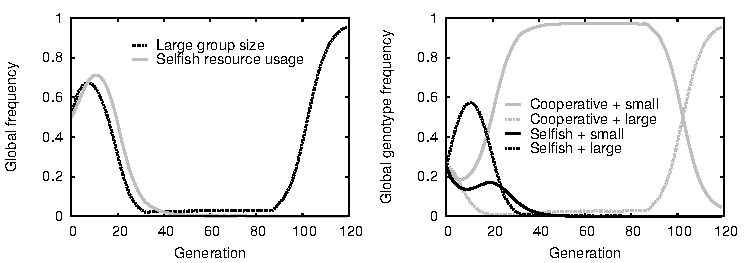
\includegraphics{sizeplot.pdf}
  \caption{Mutation on the size gene allows the cooperative + large genotype to reappear and then eventually flourish once the selfish allele has died out.}
  \label{fig:sizeplot}
\end{figure}

The initial plot was then recreated using an equal distribution of all eight genotypes, and therefore an equal proportion of mutable to non-mutable individuals - shown on these plots as a separate aggregate proportion.
\vspace{-.5cm}

\begin{figure}[!ht]
  \centering
  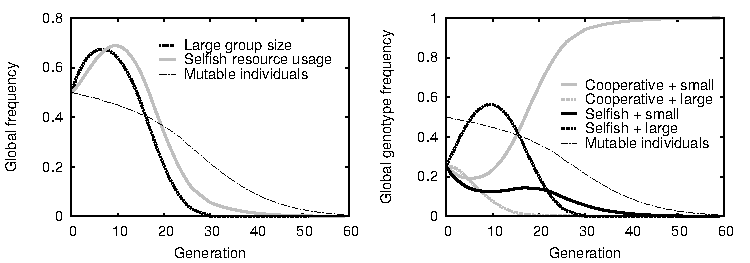
\includegraphics{60geneqmutfix.pdf}
  \caption{In this case, the addition of mutable individuals leads to the same outcome more quickly, and the mutable individuals die out.}
  \label{fig:60geneqmutfix}
\end{figure}

Finally, with a high proportion of mutable individuals it is possible to start with an inital population distribution consisting of only a single genotype, and still demonstrate the niche creation process leading to the small + cooperative genotype dominating the population.

\begin{figure}[!ht]
  \centering
  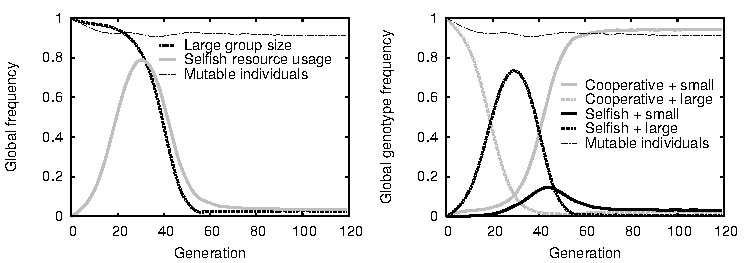
\includegraphics{120geninteresting.pdf}
  \caption{The population still contains a high proportion of mutable individuals after 120 generations, and so unlike in Figure~\ref{fig:60geneqmutfix} it is still possible that another genotype could later come to dominate, as in Figure~\ref{fig:sizeplot}.}
  \label{fig:120geninteresting}
\end{figure}

\section{Conclusion}
% ~1 page
% o  What do you conclude from that -- significance of the extension results/critique/evaluation (final page)
The addition of mutable individuals increases stochasticity - particularly for the ultimate proportion of mutable individuals. As it has no inherent effect on fitness, it is self reinforcing. Often the algorithm will select towards non-mutability as there is bias in that direction.
The increase or decrease in proportion of mutable individuals is highly self-reinforcing, and though the ultimate outcome is largely stochastic, exhibits a generally non-mutable bias.

One area for further investigation would be to allow mutation on size preference to act in a more granular manner, as suggested in \citet{thesis}. Selfish behavior
% Investigate the effects of different/a range of mutation rates

(Appendix~\ref{app:graphs}, figure~\ref{fig:further1})


\newpage
\bibliographystyle{plainnat}
\bibliography{EvoComp}{}

\newpage
\begin{appendices}
\section{Algorithm parameters}
\label{app:parameters}
\vspace{-.5cm}
\begin{table}[!ht]
  \centering
  \begin{tabular}{r|c|ccr|c}
  Behaviour parameters  & Cooperative & Selfish &  & \multicolumn{1}{c}{} & \\ \cline{1-3}
  Growth rate, $G_i$      & 0.018     & 0.02    &  & Global parameters  & Value\\ \cline{5-6}
  Consumption rate, $C_i$   & 0.1     & 0.2   &  & Population size, $N$ & 4000\\
  \multicolumn{1}{r}{} & \multicolumn{1}{c}{} & \multicolumn{1}{c}{} &  & Generations, $T$ & 120 \\
  Size parameters   & Large     & Small   &  & Reproductions, $t$~    & 4\\ \cline{1-3}
  Group size, $S_i$     & 40      & 4     &  & Death rate, $K$ & 0.1\\
  Resource influx, $R_i$    & 50      & 4     &  & \multicolumn{1}{c}{} & \\
  \end{tabular}
  \caption{Parameters from \cite{orig}, used throughout.}
  \label{table:param}
\end{table}

\section{Additional graphs}
\label{app:graphs}
\vspace{-.5cm}
\begin{figure}[!ht]
  \centering
  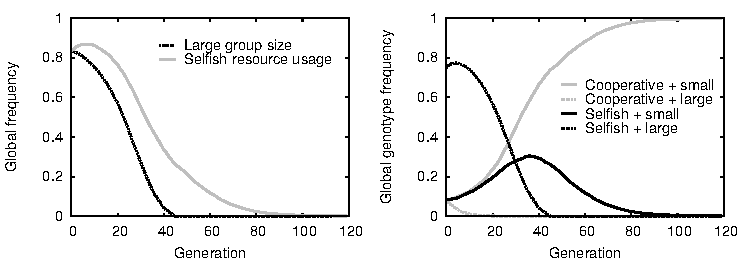
\includegraphics{unevenplot.pdf}
  \caption{The model presented in \citet{orig} is robust even in the face of severe imbalance in the initial genotype distribution.}
  \label{fig:unevenplot}
\end{figure}
\vspace{-.5cm}
\begin{figure}[!ht]
  \centering
  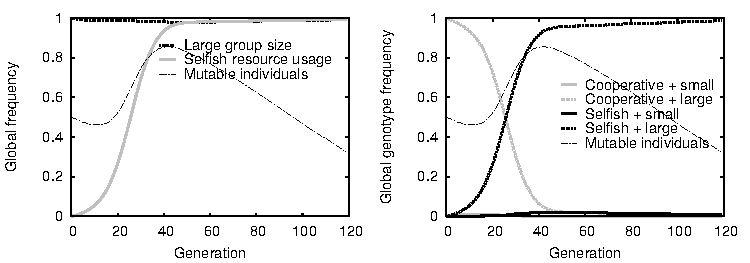
\includegraphics{further1.pdf}
  \caption{Compare to Figure~\ref{fig:120geninteresting}. The initial distributions differ only in the proportion of mutable individuals, yet provide startlingly different oucomes.}
  \label{fig:further1}
\end{figure}


\newpage
\section{Source code}
\subsection*{base.html}
\subsection*{further.html}
% Appendix: source code of what you implemented (include the source of everything you implemented as part of the pdf)
% You may also upload a zip of all source code (if this includes any code you did not implement -- it must be clearly declared in a README file, and at the front of the report)

\end{appendices}

\end{document}


What to include in your assign 2 report
See separate marks scheme for marking details.
o   Introduction: You need not spend more than 1.5 pages describing the original paper.
?         briefly describe the paper/experiment
?         What you evolved including
?         How you represented individuals
?         What fitness function did you define
?         What kind of GA you used
?         Steady state/ generational?  Tournament selection/ fitness proportionate (roulette wheel)?
?         What kind of crossover (if any) you used.
?         All parameters (enough detail so a reader could re-implement the GA)
o   Reimplementated Results (~1 page)
?         The reimplemented figures (side by side with the originals)
?         Discussion of what the results show/don't show, what worked/didn't work, what you learned
o   Describe your extension  (another page)
?        What is your research question/hypothesis?
?         e.g., 'compare x with y' or 'add x and see what difference it makes compared to not(x)'.
?         Describe methods
?         Any advancements you made
?         Support the value of asking that question (using literature)
What do you expect to happen (what might happen)?
Why do you think that?
o   Results of extension (another 1.5 page)
o  What do you conclude from that -- significance of the extension results/critique/evaluation (final page)
Appendix: source code of what you implemented (include the source of everything you implemented as part of the pdf)
You may also upload a zip of all source code (if this includes any code you did not implement -- it must be clearly declared in a README file, and at the front of the report)
 

 particular aggregation and dispersal metapopulation structure that we have modelled. 